\subsection{Câu lệnh if - elif (else if) - else}
Trong trường hợp cần xét nhiều hơn 2 điều kiện, thay vì sử dụng \texttt{else: if <condition>:}, ta có thể viết gọn thành \texttt{elif}.\par
Cấu trúc của câu lệnh if - elif - else:\par
\texttt{if <condition>:}\par
\qquad \texttt{//if block's code}\par
\texttt{elif <condition>:}\par
\qquad \texttt{//elif block's code}\par
\texttt{[elif <condition>:}\par
\qquad \texttt{//elif block's code]}\par
\texttt{[...]}\par
\texttt{else:}\par
\qquad \texttt{//else block's code}\par
\begin{figure}[h]
	\centering
	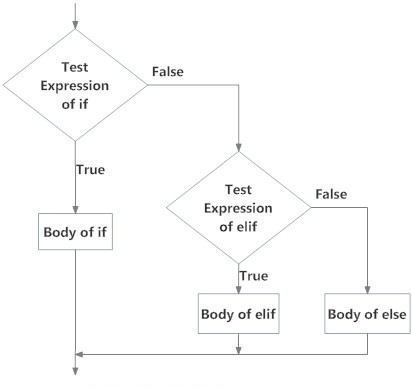
\includegraphics{img/if_elif}
	\caption{Mô tả cách thức hoạt động của câu lệnh if - elif - else}
\end{figure}
\newpage
\textbf{Ví dụ:} Chương trình nhập vào một số, kiểm tra số đó là số âm, số dương hay số 0:\\
\rule{\linewidth}{0.2mm}\par
\begin{linenumbers}
	\texttt{number = \textcolor{red}{float}(\textcolor{blue}{input}("Type a number: "))}\par
	\texttt{\textcolor{red}{if} number > 0:}\par
	\qquad \texttt{\textcolor{blue}{print}("\%.3f is a positive number." \% number)}\par
	\texttt{\textcolor{red}{elif} number < 0:}\par
	\qquad \texttt{\textcolor{blue}{print}("\%.3f is a negative number." \% number)}\par
	\texttt{\textcolor{red}{else}:}\par
	\qquad \texttt{\textcolor{blue}{print}("The number is 0.")}\par
\end{linenumbers}
\rule{\linewidth}{0.2mm}\par
\noindent
\resetlinenumber
Kết quả cho ra ở Console:\\
\rule{\linewidth}{0.2mm}\par
\begin{linenumbers}
	\texttt{Type a number: -18.25}\par
	\texttt{-18.250 is a negative number.}
\end{linenumbers}
\rule{\linewidth}{0.2mm}\par
\resetlinenumber
\newpage
\textbf{Ví dụ:} Chương trình giải phương trình bậc 2:\\
\rule{\linewidth}{0.2mm}\par
\begin{linenumbers}
	\texttt{\textcolor{red}{import} math}\par
	\bigskip
	\texttt{a = \textcolor{red}{int}(\textcolor{blue}{input}("Type your first coefficient: "))}\par
	\texttt{b = \textcolor{red}{int}(\textcolor{blue}{input}("Type your second coefficient: "))}\par
	\texttt{c = \textcolor{red}{int}(\textcolor{blue}{input}("Type your third coefficient: "))}\par
	\texttt{delta = b * b - 4 * a * c}\par
	\texttt{\textcolor{red}{if} delta < 0:}\par
	\qquad \texttt{\textcolor{blue}{print}("The equation has no solution.")}\par
	\texttt{\textcolor{red}{elif} delta == 0:}\par
	\qquad \texttt{x = - b / (2 * a)}\par
	\qquad \texttt{\textcolor{blue}{print}("x = \%.2f" \% x)}\par
	\texttt{\textcolor{red}{else}:}\par
	\qquad \texttt{x1 = (-b - math.sqrt(delta)) / (2 * a)}\par
	\qquad \texttt{x2 = (-b + math.sqrt(delta)) / (2 * a)}\par
	\qquad \texttt{\textcolor{blue}{print}("x1 = \%.2f, x2 = \%.2f" \% (x1, x2))}\par
\end{linenumbers}
\rule{\linewidth}{0.2mm}\par
\noindent
\resetlinenumber
Kết quả cho ra ở Console với ví dụ giải phương trình $2x^2 + 3x - 1$:\\
\rule{\linewidth}{0.2mm}\par
\begin{linenumbers}
	\texttt{Type your first coefficient: 2}\par
	\texttt{Type your second coefficient: 3}\par
	\texttt{Type your third coefficient: 1}\par
	\texttt{x1 = -1.00, x2 = -0.50}
\end{linenumbers}
\rule{\linewidth}{0.2mm}\par
\resetlinenumber
\newpage
\textbf{Ví dụ:} Chương trình giải hệ phương trình bậc nhất hai ẩn:\\
\rule{\linewidth}{0.2mm}\par
\begin{linenumbers}
	\texttt{a1 = \textcolor{red}{int}(\textcolor{blue}{input}("a1 = "))}\par
	\texttt{b1 = \textcolor{red}{int}(\textcolor{blue}{input}("b1 = "))}\par
	\texttt{c1 = \textcolor{red}{int}(\textcolor{blue}{input}("c1 = "))}\par
	\medskip
	\texttt{a2 = \textcolor{red}{int}(\textcolor{blue}{input}("a2 = "))}\par
	\texttt{b2 = \textcolor{red}{int}(\textcolor{blue}{input}("b2 = "))}\par
	\texttt{c2 = \textcolor{red}{int}(\textcolor{blue}{input}("c2 = "))}\par
	\medskip
	\texttt{d = a1 * b2 - a2 * b1}\par
	\texttt{dx = c1 * b2 - c2 * b1}\par
	\texttt{dy = a1 * c2 - a2 * c1}\par
	\medskip
	\texttt{\textcolor{red}{if} d == 0 and dx == dy and dx == 0:}\par
	\qquad \texttt{\textcolor{blue}{print}("This equations has an infinite number of solutions.")}\par
	\texttt{\textcolor{red}{elif} d == 0 and dx != dy:}\par
	\qquad \texttt{\textcolor{blue}{print}("This equations has no solution.")}\par
	\texttt{\textcolor{red}{else}:}\par
	\qquad \texttt{x = dx / d}\par
	\qquad \texttt{y = dy / d}\par
	\qquad \texttt{\textcolor{blue}{print}("x = \%.2f, y = \%.2f" \% (x, y))}\par
\end{linenumbers}
\rule{\linewidth}{0.2mm}\par
\noindent
\resetlinenumber
Kết quả cho ra ở Console với ví dụ giải hệ phương trình
$\begin{cases}
	x - y = 1\\
	x + y = 3
\end{cases}$:\par
\noindent
\rule{\linewidth}{0.2mm}\par
\begin{linenumbers}
	\texttt{a1 = 1}\par
	\texttt{b1 = -1}\par
	\texttt{c1 = 1}\par
	\texttt{a2 = 1}\par
	\texttt{b2 = 1}\par
	\texttt{c2 = 3}\par
	\texttt{x = 2.00, y = 1.00}
\end{linenumbers}
\rule{\linewidth}{0.2mm}\par
\resetlinenumber
\newpage